\documentclass[a4paper,11pt]{article}
\usepackage{amsmath,amsthm,amsfonts,amssymb,amscd,amstext,vmargin,graphics,graphicx,tabularx,multicol} 
\usepackage[francais]{babel}
\usepackage[utf8]{inputenc}  
\usepackage[T1]{fontenc} 
\usepackage{pstricks-add,tikz,tkz-tab,variations}
\usepackage[autolanguage,np]{numprint} 

\setmarginsrb{1.5cm}{0.5cm}{1cm}{0.5cm}{0cm}{0cm}{0cm}{0cm} %Gauche, haut, droite, haut
\newcounter{numexo}
\newcommand{\exo}[1]{\stepcounter{numexo}\noindent{\bf Exercice~\thenumexo} : \marginpar{\hfill /#1}}
\reversemarginpar


\newcounter{enumtabi}
\newcounter{enumtaba}
\newcommand{\q}{\stepcounter{enumtabi} \theenumtabi.  }
\newcommand{\qa}{\stepcounter{enumtaba} (\alph{enumtaba}) }
\newcommand{\initq}{\setcounter{enumtabi}{0}}
\newcommand{\initqa}{\setcounter{enumtaba}{0}}

\newcommand{\be}{\begin{enumerate}}
\newcommand{\ee}{\end{enumerate}}
\newcommand{\bi}{\begin{itemize}}
\newcommand{\ei}{\end{itemize}}
\newcommand{\bp}{\begin{pspicture*}}
\newcommand{\ep}{\end{pspicture*}}
\newcommand{\bt}{\begin{tabular}}
\newcommand{\et}{\end{tabular}}
\renewcommand{\tabularxcolumn}[1]{>{\centering}m{#1}} %(colonne m{} centrée, au lieu de p par défault) 
\newcommand{\tnl}{\tabularnewline}

\newcommand{\trait}{\noindent \rule{\linewidth}{0.2mm}}
\newcommand{\hs}[1]{\hspace{#1}}
\newcommand{\vs}[1]{\vspace{#1}}

\newcommand{\N}{\mathbb{N}}
\newcommand{\Z}{\mathbb{Z}}
\newcommand{\R}{\mathbb{R}}
\newcommand{\C}{\mathbb{C}}
\newcommand{\Dcal}{\mathcal{D}}
\newcommand{\Ccal}{\mathcal{C}}
\newcommand{\mc}{\mathcal}

\newcommand{\vect}[1]{\overrightarrow{#1}}
\newcommand{\ds}{\displaystyle}
\newcommand{\eq}{\quad \Leftrightarrow \quad}
\newcommand{\vecti}{\vec{\imath}}
\newcommand{\vectj}{\vec{\jmath}}
\newcommand{\Oij}{(O;\vec{\imath}, \vec{\jmath})}
\newcommand{\OIJ}{(O;I,J)}


\newcommand{\reponse}[1][1]{%
\multido{}{#1}{\makebox[\linewidth]{\rule[0pt]{0pt}{20pt}\dotfill}
}}

\newcommand{\titre}[5] 
% #1: titre #2: haut gauche #3: bas gauche #4: haut droite #5: bas droite
{
\noindent #2 \hfill #4 \\
#3 \hfill #5

\vspace{-1.6cm}

\begin{center}\rule{6cm}{0.5mm}\end{center}
\vspace{0.2cm}
\begin{center}{\large{\textbf{#1}}}\end{center}
\begin{center}\rule{6cm}{0.5mm}\end{center}
}



\begin{document}
\pagestyle{empty}
\titre{Interrogation: Triangles(3)}{Nom :}{Prénom :}{Classe}{Date}





\vspace*{0.5cm}

\exo{1.5} Cours \\

\q Donner la définition d'une médiatrice d'un triangle.\\
\reponse[3]\\

\q Quel est le point de concours des 3 médiatrices d'un triangle.\\
\reponse[2]\\

\exo{2}

\initq 
\q Construire un segment [SL] de 7,7 cm. Construire la droite (d) la médiatrice du segment [SL]. Placer un point T sur cette droite.\\

\vspace*{5cm}

\q Que peut-on dire des longueurs ST et LT ? (Justifier votre réponse)\\
\reponse[2]\\

\exo{3.5} DEF est un triangle tel que DE = 3,6 cm, DF = 6,6 cm et $\widehat{EDF}=102$.\\

\initq 

\q Construire le triangle ci-dessous et construire le cercle circonscrit à ce triangle.\\

\vspace*{7cm}






\newpage

\exo{1.5} Dans la figure ci-dessous, le point O est le centre du cercle circonscrit au triangle MPR, et les points I, J, K sont les milieux respectifs des côtés [MP], [PR] et [MR] de ce triangle.\\


\includegraphics[scale=1]{media.eps} \\


\initq
\q Quelles sont les médiatrices du triangles MPR?\\
\reponse[3]\\


\exo{1.5}\\
Voici ce qu'il reste d'un triangle ABC. I et J sont les milieux de deux côtés.\\

Sans placer les sommets B et C du triangle, construire son cercle circonscrit.\\

\vspace*{0.4cm}
\begin{center}
\includegraphics[scale=1]{triang.eps} 
\end{center}


\end{document}
